

\chapter{Implementation}

\section{Overall Design}

In our module, we can provide the PID of the process for which memory will be emulated as disaggregated memory. The module virtually divides the process memory into two parts: local memory and remote memory. The amount of local memory available in the emulator in terms of number of pages can be specified to the kernel module at the time of module insertion or dynamically using proc filesystem. The module emulates the delay whenever the remote memory is accessed by the process. This delay is the propagation and the transmission delays to fetch the remote page. We will refer both combined as "delay" in rest of the report. Transmission delay is calculated based on bandwidth of the network and the size of the page that is being fetched. Propagation delay and bandwidth can be provided at the time of module insertion or dynamically via configured proc files. 


\section{Memory Management in Linux}

Since module has to inject the delay at a memory access, page fault handler is the place where we can put the delay logic. There are various reasons to trigger page fault in linux kernel. The MMU hardware (Figure\ref{fig:mmu}) is responsible for process memory address translation. MMU uses an internal page table to lookup page table entry (PTE) corresponding to a virtual address. This PTE is used to find the physical address for a given virtual address. PTE also stores various flags. Table \ref{tab:pte_flags} shows flags set in PTE.

\begin{figure}[tbp]
  \centering
    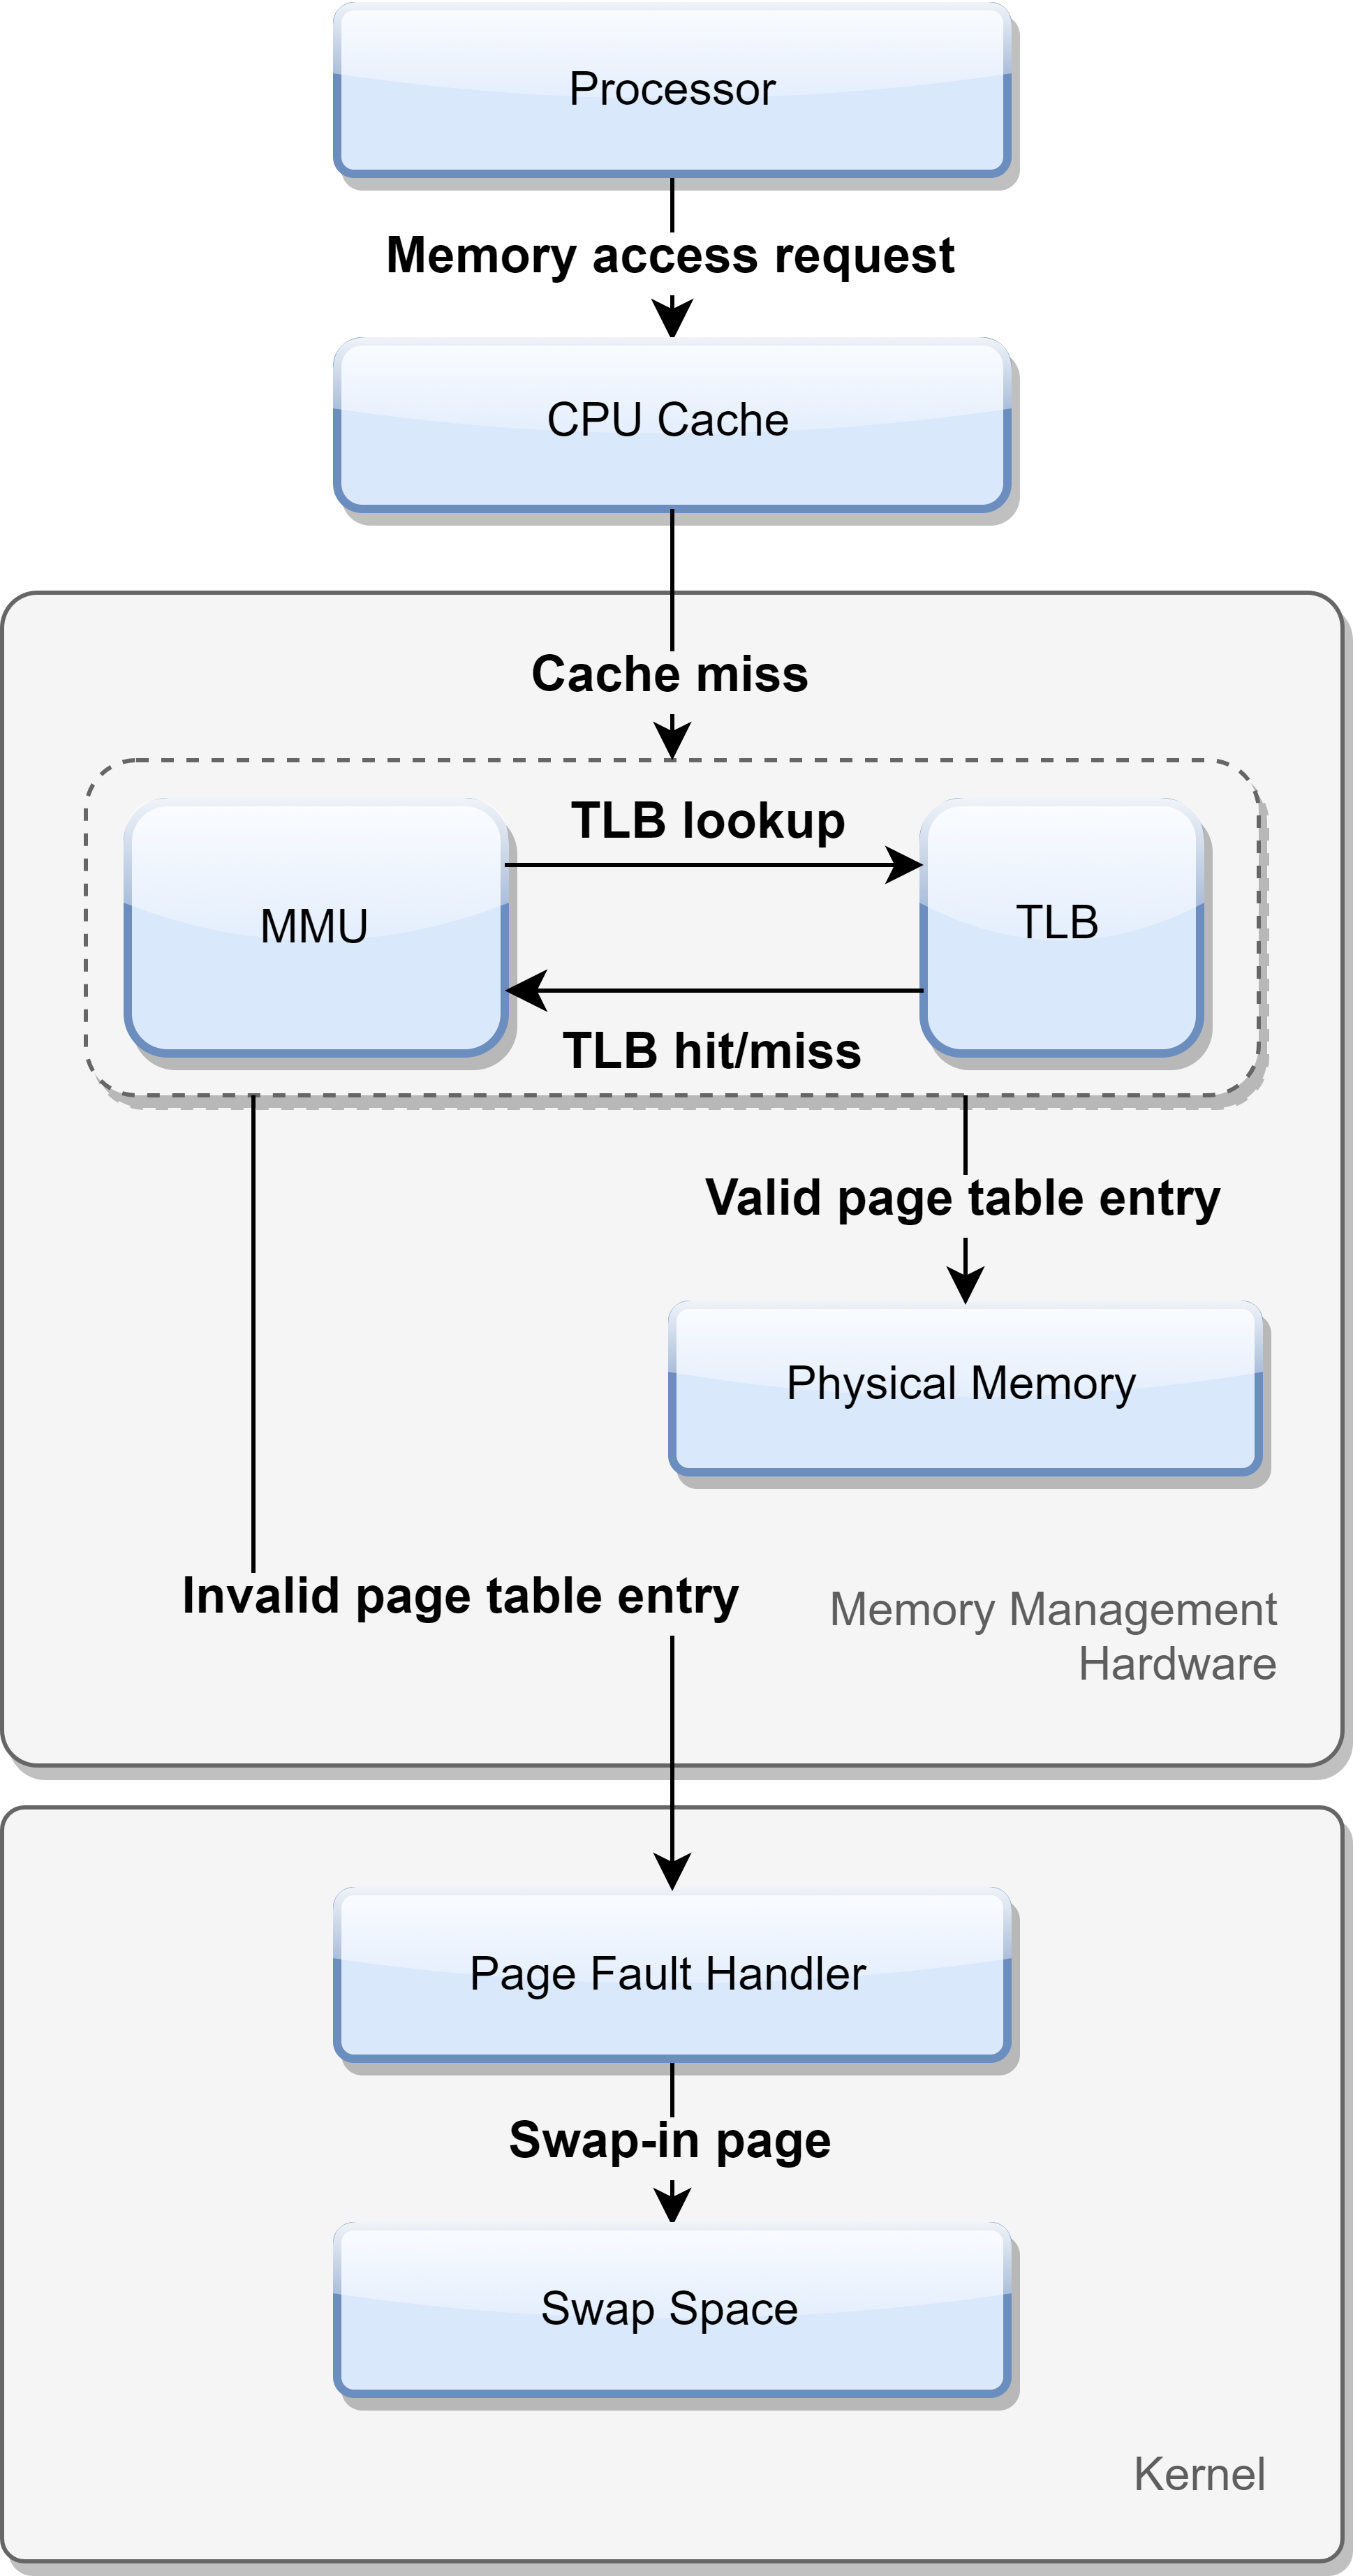
\includegraphics[width=0.5\textwidth]{implementation/mmu}
    \caption[MMU hardware]{MMU and page fault handler interaction.}
    \label{fig:mmu} 
\end{figure}


\begin{table}[tbp]
  \centering
    \caption{PTE flags.}
    \label{tab:pte_flags}
    \begin{tabular}{ll}
      \toprule 
      Bit & Function \\
      \midrule
      \verb|_PAGE_PRESENT| & Page is resident in memory and not swapped out \\
      \verb|_PAGE_PROTNONE| & Page is resident but not accessable \\
      \verb|_PAGE_RW| & Set if the page may be written to \\
      \verb|_PAGE_USER| & Set if the page is accessible from user space \\
      \verb|_PAGE_DIRTY| & Set if the page is written to \\
      \verb|_PAGE_ACCESSED| & Set if the page is accessed \\
      \bottomrule \\
    \end{tabular}  
\end{table}

When MMU cannot serve the address translation request, a page fault is raised. CPU breaks the normal program execution flow and handles the raised fault. In x86 architecture, function named "\verb|do_page_fault|" in file "arch/x86/mm/fault.c" in kernel source code handles the page fault.

There are various reasons for triggering a page fault. We are going to focus on following reasons:
\begin{enumerate}
    \item Page was never loaded into the memory, i.e. first reference to the address within the page: demand paging
    \item Page is present in memory and protection bit is set in PTE
    \item Page was swapped-out from memory
\end{enumerate}

If MMU is able to translate the virtual address successfully, no fault is raised and program flow is not interrupted.


\section{Emulator Workflow}

To inject the delay to each page fault, the module follows the steps :
\begin{enumerate}
    \item Intercepts each page fault
    \item Determine if the page fault is raised for a process for which the emulation is running
    \item Determine if the faulted address is in the local memory or the remote memory
    \item No delay injection if address belongs to local memory
    \item If address is in remote memory, virtually allocate a local page
    \begin{enumerate}
        \item If local memory pool is free, virtually allocate the new local page to the faulted page
        \item Else virtually evict a page from local memory pool and allocate the the new freed slot to the faulted page
    \end{enumerate}
    \item Inject the delay for emulating the transmission and propagation delays
\end{enumerate}



\section{Induce Page Faults}

A page fault can be induced by setting the \verb|_PAGE_PROT_NONE| bit and resetting \verb|_PAGE_PRESENT| bit of PTE of the required page. This combination of bits prevents page fault handler from behaving unexpectedly. It suggests that the page is present in memory but access to it is protected. Setting the above combination of flags is referred as protecting the page and setting opposite combination of flags (i.e. \verb|_PAGE_PROT_NONE|=0 \& \verb|_PAGE_PRESEN|=1) is referred as releasing the page in rest of the report for simplicity.
Kernel module sets this flags combination for all PTEs of the process with given PID when it gets inserted into the kernel. This way every memory access by the given process will trigger the page fault.

\section{Intercept a Kernel Function}
Module needs to intercept each page fault so that it can emulate the delay. There are two ways to intercept a kernel function:
\begin{enumerate}
    \item KProbe
    \item Kernel hooks
\end{enumerate}

\subsection{KProbe}

KProbe is a debugging mechanism provided by the kernel to track the activities inside the kernel. It allows to set breakpoints in running kernel. A kprobe can be added to any function whose address is known at the time of kprobe insertion. Kernel recompilation is not needed in this method.

But \verb|do_page_fault| function is tagged with "\verb|NOKPROBE_SYMBOL(fname)|" macro, which disables kprobe for the given function. To avoid calling any kind of tracing machinery before the function has observed the CR2 value.

\subsection{Kernel hooks}
Adding a hook to the kernel function is another way of intercepting a kernel function, but with added overhead of recompilation of the kernel.  We have added a hook function pointer in \verb|fault.c| file initialized to null value. We are calling the hook function before \verb|__do_page_fault| function in \verb|do_page_fault| function. The hook function is called only if the function pointer is not null. The hook function pointer is exported so that the kernel module can set its value to pointer to custom function defined inside the module. Module sets the hook function pointer back to null at the time of module removal, to prevent invalid memory access.

\begin{figure}[tbp]
  \centering
    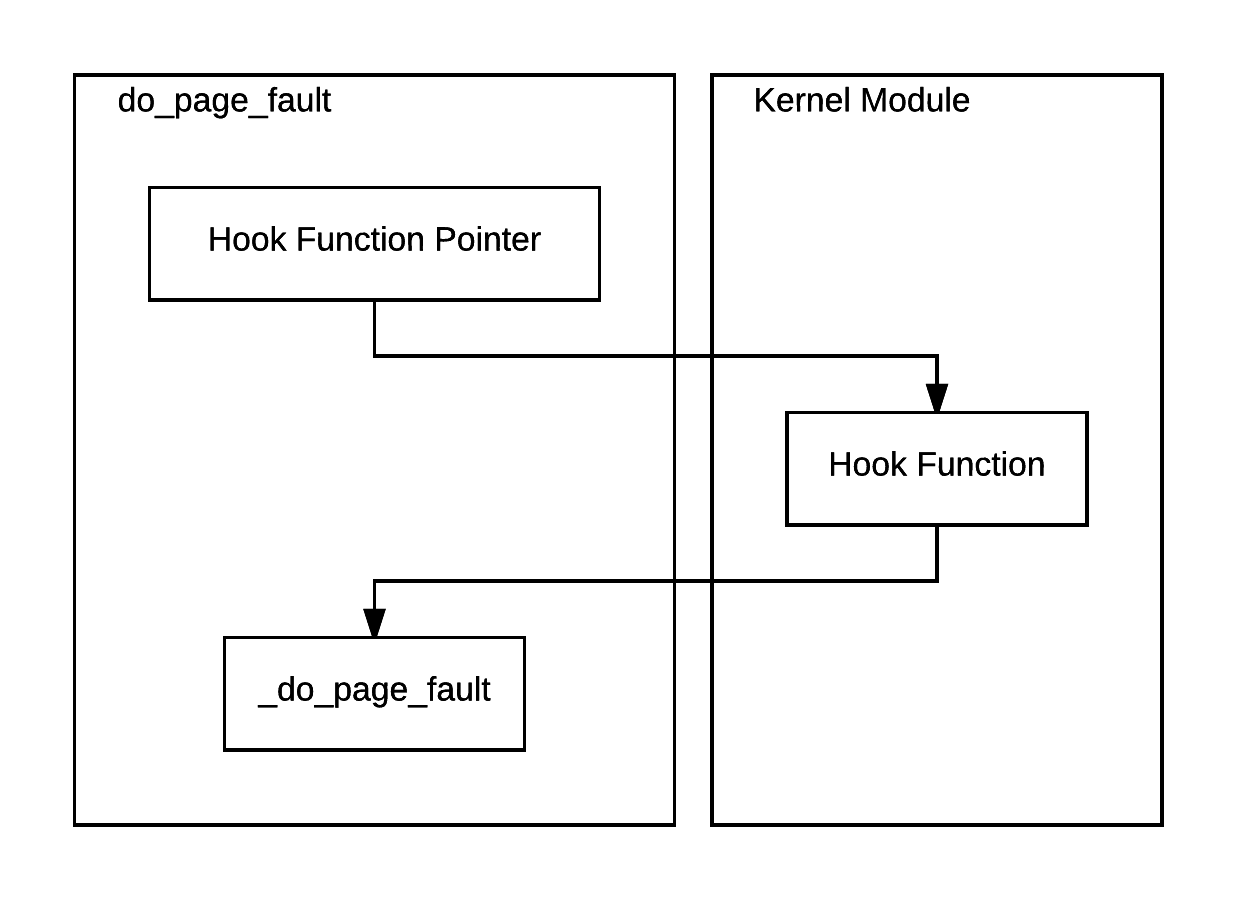
\includegraphics[width=0.7\textwidth]{implementation/hook}
    \caption[Hook Function]{Hooking a page fault handler function.}
    \label{fig:hook_1} 
\end{figure}


Kernel module first initializes the required data structures then sets the hook function pointer and then sets the PTE flags combination as described above, so that it does not miss any page fault.

\section{Delay Execution}
Now we have setup the page fault interception and induced the page fault for every memory access from the insertion of our module, which is our first step. The delay injection logic is implemented in the hook function defined in the module.


\subsection{PID of faulted process}
Now to determine the process which has triggered the page fault, hook uses \verb|current| macro to get \verb|task_struct|. PID is extracted from \verb|task_struct| which is compared with the PID provided at the time of module insertion. The hook function returns without doing anything if the PID does not match.


\subsection{Virtual memory location}
Next step is to determine virtual location of faulted page, i.e. if it is local memory or remote memory.

The module maintains a list of "local" pages, i.e. list of address of the pages which are virtually at the local memory for the process. Local page list helps to select a local page for eviction. When a remote page is brought to local memory, its address is added to the local page list. The page is released so that future address reference would not trigger the page fault. For evicting a local page, the page address is removed from the local page list and the page is protected, so that any future reference to that page would trigger the page fault and the hook function can inject the delay.

Now as the setup suggests, the page fault will trigger only for remote pages, we don't need to traverse the local page list to determine the virtual location of the page. So for every page fault for that process, hook will inject the delay.

This way emulator does not inject the delay for the pages which are in the list, but all other pages. Local page list also helps to select a local page for eviction.

Hook decides to remove a page from the local page list if the local memory is virtually full, i.e. the count of the pages in local page list has reached the max local memory specified during module insertion. 
After removing a local page from list, faulted page is inserted into the list, then hook executes the delay and returns.

We discuss a special scenario later in the document, where we must traverse the list to determine virtual page location. 
Currently the module does not check if the page is in the local page list. It requires a data structure which will help fast lookup and update. This feature is discussed in future work section.



\section{Second Hook}

\subsection{Accurate delay execution}
The hook function can take variable amount of time to reach at the delay execution code based on the various tasks it needs to complete, e.g. local page lookup, update, etc. Also, \verb|__do_page_fault| function can take variable time to return based on the type of page fault. Therefore, there will be variable amount of delay injection for each page fault.

To be able to inject the exact amount of delay based on the calculation, the module must calculate the time spent on these extra tasks and inject delay worth of the difference of desired delay and time spent.
To achieve the accurate delay execution, we need another hook function which will be called at the end of \verb|do_page_fault| function. Now the first hook function will take the timestamp as a start of the handler and the second hook function will execute the difference worth of delay at the end.

The timestamp variable must be accessible from both hook functions, but it should not be taken as a global variable, since there might be multiple page faults being handled at the same time. So, we declare a timestamp variable in \verb|do_page_fault| function, whose single instance will be common for both hook functions but different for each page fault.

\subsection{Delay execution decision}
Since there are reasons for which a page fault could occur other than our page protection, e.g. demand paging, swapped-out page. First hook function should decide whether to execute the delay and second hook should execute the delay based on this decision. 
Now again since both hooks are different functions, we cannot have a global flag variable for the decision communication. So, same as timestamp, we declare a flag variable in \verb|do_page_fault| and its pointer is sent to both hooks as an argument.

\begin{figure}[tbp]
  \centering
    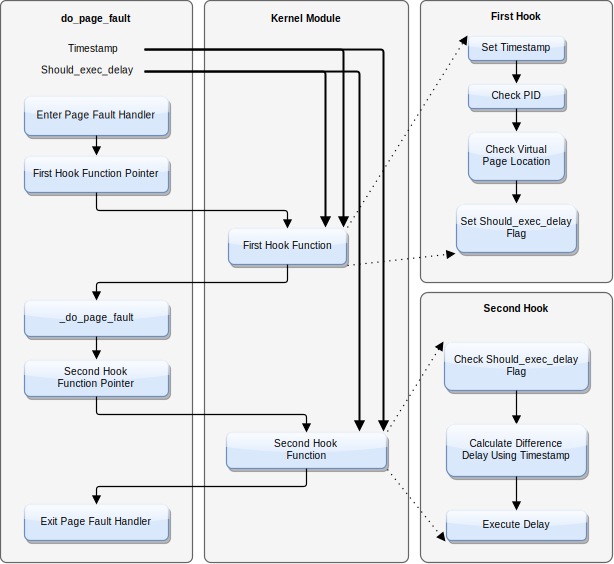
\includegraphics[width=1.0\textwidth]{implementation/second_hook}
    \caption[Second Hook Function]{Emulator with second hook.}
    \label{fig:hook_2} 
\end{figure}


\section{Tyeps of Page Faults}

\subsection{Minor Page Faults}

A minor page fault occurs only when the page list is updated (and the MMU configured) without actually needing to access the disk. This happens when a page is shared across processes but current process does not have access for it, e.g. in case of same binary is executed by different users. 
Another example is copy on write. When a new process is forked, the child process shares the address space of parent process. A separate copy of the page is created only when a write operation happens on the shared page.
Both of these page faults has less work to do and page fault occurs only once for that page.

\subsection{Demand paging}
In this case, the page is not present in physical memory and kernel should allocate the page or load the page from disk.
The \verb|_PAGE_PRESENT| flag is not set in PTE. So we can simply add these pages to local page list and execute delay. Two page faults are triggered for this case. First page fault starts loading and allocating the page and second page fault initialises PTE. The \verb|_PAGE_PRESENT| bit is not set in first page fault, but it is set in second page fault. So by checking \verb|_PAGE_PRESENT| only, we can serve multiple page faults for a page only once.

\subsection{Swap-in Pages}

When a page is swapped-in into the memory, its \verb|_PAGE_PROT_NONE| and \verb|_PAGE_PRESENT| flags are reset. So the module has no idea about whether the page was in local page list or not. The only way to find out that is to traverse the list. The size of the list could be very large depending on max number of allowed local pages. Same as demand paging, this type of page fault also triggers two page faults.

There are extra unused bits (\verb|_PAGE_BIT_SOFTW{1,2,3,4}|) of PTE in x86 architecture. We tried setting these bits to represent if page is in local memory or remote memory, but same as \verb|_PAGE_PROT_NONE| bit, they also gets cleared when page gets swapped-in.

Currently we are ignoring this scenario. Current module treats all pages as remote pages for which \verb|_PAGE_PRESENT| is not set and executes delay. This leads to multiple entries in the local page list, which is not the serious problem but the emulation will not be accurate.
Solution for this problem is discussed in future work section.


\begin{table}[tbp]
  \centering
    \caption{PTE flags and corresponding type of page fault.}
    \label{tab:pte_flags_vs_type} 
    \begin{tabular}{cc|p{.2\textwidth}|p{.3\textwidth}}
    \toprule 
	\multicolumn{2}{c|}{Bits} &  
	\multirow{2}{*}{Type} & \multirow{2}{*}{Action} \\
%	\cline{1-2}
	\_PAGE\_PRESENT& \_PAGE\_PROT\_NONE & &     \\
    \midrule	
	0 & 0 &  Page not present in physical memory & 
	Check page in local page list, add if not present and emulate delay		
	\\ \hline		
	0 & 1 &  
	Page is present but protected 		&  
	Add to local page list and emulate delay \\ 
	\hline	
	1   & 0     & Page is loaded in physical memory, but not initialized & Ignore page fault, since page is already in local page list
	\end{tabular}
\end{table}


\chapter{Verification of Correctness}

We have written a test program in C language, which takes number of pages as an argument and "malloc"ates the memory. Since we have disabled huge pages, default page size is 4kB. The program accesses all the allocated pages in sequence. At the end of execution, test script extracts total number of page faults occurred from module parameter \verb|page_fault_count|. 

Expected delay per page fault is calculated using module parameters provided (Shown in Table \ref{tab:kmodule_param}). Actual delay per page is computed by dividing total execution time with \verb|page_fault_count|. 




\begin{table}[tbp]
	\centering
	\caption{Emulator module parameters.}
	\label{tab:kmodule_param}
	\begin{tabular}{lll}
		\toprule 
		Parameter Name & Access & Use \\
		\midrule
		\verb|pid| 				& Read Only 	& PID of process to emulate, set at the time of module insertion \\
		\verb|latency_ns| 		& Read/Write	& One way propogation delay in nano-sec \\
		\verb|bandwidth_bps| 	& Read/Write	& Bandwidth of the network \\
		\verb|local_npages| 	& Read/Write	& Local memory interms of number of pages \\
		\verb|page_fault_count| & Read Only		& Total number of page faults \\
		\bottomrule
	\end{tabular}  
\end{table}

Table \ref{tab:test_results} shows the test results with different number of allocated pages in test program. Number of page faults are grater than total number of pages allocated even the test program accesses each page only once. This is because local pages are evicted as local memory gets full. Since we are using FIFO policy instead of LRU for eviction, pages containing execution code gets protected after every \verb|local_npages| page faults. Because of this page fault count gets a boost.


\begin{table}[tbp]
	\centering
	\caption{Emulator module parameters.}
	\label{tab:test_results}
	\begin{tabular}{llll}
		\toprule 
		\# of allocated pages 	& Page fault count 	& Expected delay per page 	& Actual delay per page \\
		\midrule
		500 		& 564 		& 40.00 ms	& 	39.00ms \\
		1000 		& 1103 		& 40.00 ms	& 	43.00ms \\
		10000 		& 10156 	& 40.00 ms	& 	44.00ms \\
		100000 		& 100697	& 40.00 ms	& 	44.00ms \\
		1000000 	& 1006127 	& 40.00 ms	& 	43.00ms \\
		\bottomrule
	\end{tabular}  
	\medskip
	\small
	Following module parameters were set for testing:
	
	\verb|latency_ns|=20000 ns;
	\verb|bandwidth_bps|=10000000000000000 bps;
	\verb|local_npages|=1000.
\end{table}


\chapter{Future Work}

\section{Fast local page list lookup}
Based on our tests, we found that when a page is swapped-in, all PTE flags are reset. We need to lookup the local page list if the page was in local memory space before it got swapped-out. Only way currently we see is to traverse the local page list. A fast mechanism to lookup if a given page is in local page list is required for every swapped-in page. A hash table can be used to maintain list of local pages.

More efficient method will be explored in parallel.

\section{Local page replacement policy}
A more efficient and accurate in terms of which emulates actual architecture algorithm for local page replacement policy is required. Currently FIFO policy is used.

\section{Fine grained control}
A fine grained control over location of memory range which can be provided dynamically using proc filesystem. A process can also use custom malloc function which uses extra flag argument which suggests location of the memory allocated. Dynamically flush a range of local memory. Dynamically set number of local pages.

\section{Support for huge pages}
Currently we are disabling huge pages in linux. We can enable huge pages and execute accurate transmission delay based on page size being transferred.

\section{Process groups}
To be able to add/remove multiple processes to the emulator dynamically. Automatically add child process to the emulator when forked.


%%% Local Variables: 
%%% mode: latex
%%% TeX-master: "../mainrep"
%%% End: 
